\documentclass[]{article}

\usepackage[margin=0.85in]{geometry}

\usepackage{fontawesome5}
\usepackage{fancyhdr}
\usepackage{lastpage}
\usepackage{amssymb}
\usepackage{halloweenmath}
\usepackage{multicol}
\usepackage{ragged2e}

\usepackage{xcolor}
\definecolor{light-gray}{gray}{0.25}

\usepackage{hyperref}
\hypersetup{
    colorlinks=true,
    linkcolor=violet,
    filecolor=black,      
    urlcolor=violet,
    citecolor = black
}

\usepackage{enumitem}
\setitemize{itemsep=0pt, itemindent=10pt}

% Reference formatting
\newlength{\cslhangindent}
\setlength{\cslhangindent}{1.5em}
\newenvironment{cslreferences}
{\setlength{\parindent}{0pt}
\everypar{\setlength{\hangindent}{\cslhangindent}}\ignorespaces}
{\par}

%title formatting
\usepackage{titlesec}
\titleformat{\section}[block]{\bfseries\sc}{}{1.2em}{}
%\titleformat{\section}[block]{\Large\bfseries\filcenter}{}{1em}{}
\titleformat{\subsection}[hang]{\bfseries}{}{1em}{}
\setcounter{secnumdepth}{0}

\titlespacing*{\section}
{0pt}{12pt}{3pt}
\titlespacing*{\subsection}
{0pt}{10pt}{3pt}

%For LIST spacing
\providecommand{\tightlist}{%
  \setlength{\itemsep}{0pt}\setlength{\parskip}{0pt}}

%Set paragraph indent and between paragraph spacing
\setlength\parindent{0pt}
\setlength{\parskip}{0pt}

% Widow and orphan prevention
\widowpenalty10000
\clubpenalty10000

%Need all these for graphics and tables
\usepackage{subfig}
\usepackage{graphicx}
\usepackage{blindtext}
\usepackage{array}
\usepackage{wrapfig}
\usepackage{wallpaper}
\usepackage{lmodern}

\usepackage[pages=some]{background}
\backgroundsetup{
scale=1,
color=black,
opacity=0.35,
placement=top,
hshift=24,
vshift=-20,
%position={5cm,7cm},
angle=0,
contents={%
  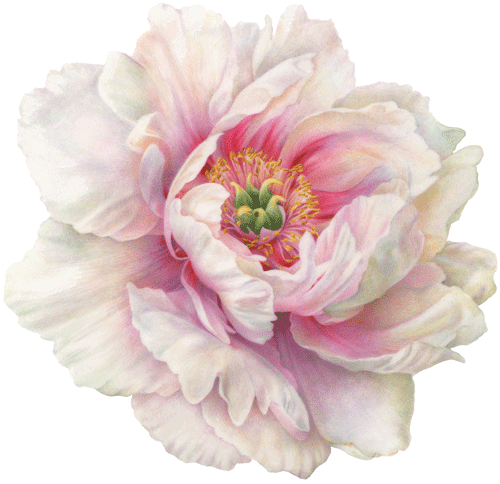
\includegraphics[width=0.25\textwidth]{images/peony.png}
  }%
}


\pagestyle{fancy}
\fancyhf{}
\fancypagestyle{firstpage}{%
\renewcommand{\headrulewidth}{0pt}
\fancyhead[R]{\href{mailto:ldelan5@uic.edu}{ldelan5@uic.edu} \faPaperPlane\\
\href{https://ledelaney.org}{ledelaney.org} \faLaptop}
\fancyfoot[R]{\footnotesize{\today\ $\vert$ page \thepage\ of \pageref{LastPage}}\\
\footnotesize{L E Delaney \href{https://github.com/ledelaney/led-cv}{\faGithub}}}}

\fancypagestyle{alldocument}{
\renewcommand{\headrulewidth}{0pt}
\fancyhead[R]{}
\fancyfoot[R]{\footnotesize{\today\ $\vert$ page \thepage\ of \pageref{LastPage}}\\
\footnotesize{L E Delaney \href{https://github.com/ledelaney/led-cv}{\faGithub}}}}


\begin{document}
\BgThispage
\pagestyle{alldocument}

%\begin{center}
{\fontsize{20}{64}\selectfont \textsc{Lucy E Delaney}}\\

% \vspace{1mm}
% {\fontsize{15}{64}\selectfont \textsc{Graduate Student in Biological Sciences}}\\
% \vspace{1mm}
% {\fontsize{15}{64}\selectfont University of Illinois at Chicago}\\
%\end{center}
\leftskip 5em
\begin{multicols}{2}

University of Illinois at Chicago\\
Department of Biological Sciences\\
Chicago, IL 60607

\columnbreak

\begin{flushright}
\rightskip 5em
\href{mailto:ldelan5@uic.edu}{ldelan5@uic.edu} \textcolor{light-gray}{\faPaperPlane}\\
\href{https://github.com/ledelaney}{@ledelaney} \textcolor{light-gray}{\faGithub}\\
\href{https://ledelaney.org}{ledelaney.org} \textcolor{light-gray}{\faDesktop}
\end{flushright}

\end{multicols}

\vspace{0.5mm}

\section{Interests}
\vspace{3mm}

\leftskip 1.8em

Conceptual understanding of evolutionary principles, evolution-centered teaching of biology, educational \& racial equity, \textcolor{light-gray}{\faRProject}\ for undergraduate education, macroevolution, the evolution of plant breeding systems

\section{Education}

\vspace{4mm}
\leftskip 1.8em

\textbf{Ph.D. candidate, Ecology \& Evolutionary Biology} \hfill \textit{Expected 2022}\\ 
University of Illinois at Chicago \hfill Chicago, IL
     
Dissertation: \emph{The Nature of Adaptation and the Epistemology of Natural Selection} 
\vspace{0.3cm}

\textbf{M.A., Molecular \& Cellular Biology} \hfill 2016\\ 
Hunter College of the City University of New York \hfill New York, NY\\
     

\textbf{B.S., Forensic Molecular Biology, Philosophy} \hfill 2012\\ 
John Jay College of the City University of New York \hfill New York, NY

\section{Skills}

%\leftskip 1.8em

\begin{multicols}{3}
\begin{itemize}
	\item[\textcolor{light-gray}{\faRProject}]{\texttt{R} and \texttt{RMarkdown}}
	\item[\textcolor{light-gray}{\faBroadcastTower}]{Technician radio license}
	\item[]{}
\end{itemize}

\columnbreak

\begin{itemize}
	\item[\textcolor{light-gray}{\faFilePdf}]{\LaTeX\ and \DeclareRobustCommand{\BibTeX}{%
  {\normalfont B\kern-.05em{\scshape i\kern-.025em b}\kern-.08em \TeX}%
}\BibTeX}
\item[\textcolor{light-gray}{\faFileCode}]{\texttt{HTML} and \texttt{CSS}}
\item[\textcolor{light-gray}{\faFilePrescription}]{Shell scripting (novice)}
\end{itemize}

\columnbreak

\begin{itemize}
	\item[\textcolor{light-gray}{\faDraftingCompass}]{Adobe Illustrator}
	\item[\textcolor{light-gray}{\faMicrosoft}]{Microsoft Office Suite}
	\item[]{}
\end{itemize}

\end{multicols}


\section{University Teaching}

\vspace{4mm}
\leftskip 1.8em

\textbf{BIOS 220} Mendelian and Molecular Genetics \hfill Fall 2019--Summer 2020
     
Sophomore-level course focusing on Mendelian inheritance patterns and molecular mechanisms of \linebreak inheritance. Helped managed transition from in-person to online delivery. Responsible for teaching discussion section, creating digital course materials \& exams, grading, drop-in hours, and Blackboard \linebreak administration. \href{https://ledelaney.org/teaching/genetics220/}{\faLink} \href{https://github.com/ledelaney/Genetics220}{\faGithub}\\
     
\textbf{BIOS 331} General Ecology Laboratory \hfill Summer 2019

Application of ecological and evolutionary concepts with hands-on experiments and field trips to local natural areas. Responsible for weekly laboratory instruction, drop-in hours, and grading. \href{https://github.com/ledelaney/GeneralEcologyMaterials}{\faGithub}\\
     
\textbf{BIOS 230} Ecology and Evolution \hfill Spring 2019

Sophomore-level course with emphasis on basic ecological systems, ecosystem dynamics, and \linebreak evolutionary principles. Responsible for weekly office hours, assignment creation, and grading.\\
     
\textbf{BIOS 430} Evolution \hfill Fall 2017--Fall 2018
     
Upper-division, programming-focused course on evolutionary theory and principles. Responsible for weekly drop-in hours \& debugging, quiz materials, and grading of \textcolor{light-gray}{\faRProject}\ programming assignments.\\

\textbf{BIOS 120} Biology of Populations and Communities \hfill 2016--2017
     
Introductory biology laboratory course with emphasis on ecological and evolutionary principles. \linebreak Responsible for twice-weekly laboratory instruction, drop-in hours, and grading.

\clearpage
\pagestyle{alldocument}

\section{Community Teaching}
\vspace{4mm}
\leftskip 1.8em

\textbf{Course Builder \& Trainer} UIC Biological Sciences Department \hfill 2020--Present
     
Trained in online instructional design \& pedagogy, and software relevant to online teaching \& \linebreak learning. Assisting Biological Sciences Department faculty members in transitioning their courses online, and managing technical aspects of courses throughout online delivery. Creator and maintainer of the UIC Course Builder Website. \href{https://www.ledelaney.org/cb-materials}{\faLink} \href{https://github.com/ledelaney/cb-materials}{\faGithub}\\
     
\textbf{Tutor} Nurturing Wisdom Tutoring \hfill 2018--2020
     
Highly-rated individual tutoring for grades 7-12 in test preparation (SAT and high school entrance \linebreak exams), science, mathematics, and writing.\\

\textbf{Substitute Teacher} Chicago-area Charter Schools \hfill 2015-2016
     
Substitute teacher for elementary, middle, and high school classes.

\section{Teaching Honors and Awards}

\vspace{4mm}
\leftskip 1.8em

\begin{itemize}[label=$\mathwitch*$]
\item{\textbf{2021} Honorable mention, UIC Graduate Student Excellence in Teaching and Mentoring Award}
\item{\textbf{2020} Recipient, Biological Sciences Department Graduate Teaching Award for BIOS 220}
\item{\textbf{2018} Recipient, Biological Sciences Department Graduate Teaching Award for BIOS 430}
\end{itemize}

\section{Past and Upcoming Presentations}

\vspace{4mm}
\leftskip 1.8em

\textit{\textbf{Natural Selection Does Not Come Naturally}}

\begin{itemize}[label=$\mathwitch*$]
\item{June 2021 \textit{upcoming} at Annual Evolution Conference $\vert$ Virtual Talk 
\hspace{0.3mm} \href{https://ledelaney.org/talks/2021evolution}{\faImages} \href{https://github.com/ledelaney/06-21-Evolution}{\faGithub}}
\end{itemize}
\vspace{2mm}

\textit{\textbf{The Four Causes of Adaptation}}

\begin{itemize}[label=$\mathwitch*$]
\item{March 2021 at Midwest Ecology and Evolution Conference $\vert$ Awarded Best Graduate Talk \hspace{0.3mm} \href{https://twitter.com/MEEC2021/status/1373669196966543360?s=20}{\faAward} \href{https://ledelaney.org/talks/2021meec/}{\faImages} \href{https://github.com/ledelaney/03-21-MEEC}{\faGithub}}
\item{January 2021 at SABER West $\vert$ Virtual Roundtable \hspace{0.3mm} \href{https://ledelaney.org/talks/2021saberw/}{\faImages} \href{https://github.com/ledelaney/01-21-SABERwest}{\faGithub}}
\end{itemize}
\vspace{2mm}


\textit{\textbf{The Phylogenetic Distribution and Frequency of Self-Incompatibility in Fabaceae}},\\ with Ramanauskas, K. \& Igić, B.

\begin{itemize}[label=$\mathwitch*$]
\item{July 2021 \textit{upcoming} at Annual Meeting of the Botanical Society of America $\vert$ Virtual Talk}
%\hspace{0.3mm} \href{https://ledelaney.org/talks/meectalk/MEEC-slides.html}{\faImages} \href{https://github.com/ledelaney/03-21-MEEC}{\faGithub}}
\item{July 2018 at Annual Meeting of the Botanical Society of America $\vert$ Rochester, MN $\vert$ Poster \hspace{0.3mm} \href{https://ledelaney.org/static/posters/poster.png}{\faFileImage}}
\end{itemize}
\vspace{2mm}

\textit{\textbf{Evolutionary Consequences of Plant Mating Systems}}

\begin{itemize}[label=$\mathwitch*$]
\item{August 2017 at microMORPH Summer Course $\vert$ Arnold Aborteum, Harvard $\vert$ Talk \hspace{0.3mm} \href{https://www.dropbox.com/s/o7hcg5riw97wf9i/08-2017-microMORPH.pdf?dl=1}{\faImages}}
\end{itemize}
\vspace{2mm}

\section{Publications}

\vspace{4mm}
\leftskip 1.8em

\begin{cslreferences}
\textbf{Delaney, Lucy E}. (2012). Nietzsche, nerve stimulation-image connection, and ontology. \emph{John Jay's Finest}, \emph{27}, 99--103. \href{https://ledelaney.org/static/docs/Delaney-JJAYFinest.pdf}{\faFile}\\
\end{cslreferences}

\subsection{\textit{In preparation}}
\vspace{2mm}

\begin{cslreferences}
\textbf{Delaney, Lucy E}, Ramanauskas, K., \& Igić, B. The phylogenetic distribution and frequency of self-incompatibility in Fabaceae: What do we know?

\textbf{Delaney, Lucy E} \& Igić, B. The orchids and their breeding systems.\\
\end{cslreferences}

\section{Other Awards and Training}

\vspace{4mm}
\leftskip 1.8em

\begin{itemize}[label=$\mathwitch*$]
\item{\textbf{2020} Participant in the 2020 Chicago \textcolor{light-gray}{\faRProject}\ Collaborative Conference \href{https://chircollab.github.io/}{\faLink}}
\item{\textbf{2018} Recipient of the Biological Sciences Department Travel Award}
\item{\textbf{2018} Reviewer for International Journal of Botany, Oxford Bibliographies}
\item{\textbf{2017} Accepted to NSF-funded workshop on Bayesian Analysis of Macroevolutionary Mixtures \href{http://bamm-project.org/index.html}{\faLink}}
\item{\textbf{2017} Recipient of the Biological Sciences Department Travel Award}
\item{\textbf{2017} Accepted to microMORPH Plant Anatomy Summer Course at Harvard University \href{https://web.archive.org/web/20170922060558/http://arboretum.harvard.edu/tracing-evolution-form-function/"}{\faLink}}
\item{\textbf{2016} General horticulture volunteer at Garfield Park Conservatory \href{https://garfieldconservatory.org/}{\faLink}}
\end{itemize}

\section{Professional Experience}

\vspace{4mm}
\leftskip 1.8em

\textbf{Forensic Molecular Biologist} at NYC Office of Chief Medical Examiner \hfill 2012--2015
     
Examined evidence for the presence of biological fluids, performed serological \& DNA analysis \linebreak techniques, analyzed data \& performed statistical analyses, wrote reports, and provided expert \linebreak scientific testimony in court.\\
   
\textbf{Health Research Intern} at NYC Department of Health \hfill 2011-2012
     
Accepted to the Health Research Training Program for a year-long internship with the Bureau of \linebreak Environmental Disease Prevention. Received training in disease epidemiology, emergency preparedness \& response, public health and outreach programs in environmental disease control \&  prevention, and emerging viral infections.\\
     
\textbf{Field Manager \& Administrative Assistant} at Working Families Party \hfill 2008-2011
     
Responsible for payroll, managing employees' healthcare coverage, bank deposits, and data entry. \linebreak Organized informational events for the public, and served as Field Manager for multiple election and fundraising campaigns.

\end{document}